% Options for packages loaded elsewhere
\PassOptionsToPackage{unicode}{hyperref}
\PassOptionsToPackage{hyphens}{url}
%
\documentclass[
]{article}
\usepackage{amsmath,amssymb}
\usepackage{iftex}
\ifPDFTeX
  \usepackage[T1]{fontenc}
  \usepackage[utf8]{inputenc}
  \usepackage{textcomp} % provide euro and other symbols
\else % if luatex or xetex
  \usepackage{unicode-math} % this also loads fontspec
  \defaultfontfeatures{Scale=MatchLowercase}
  \defaultfontfeatures[\rmfamily]{Ligatures=TeX,Scale=1}
\fi
\usepackage{lmodern}
\ifPDFTeX\else
  % xetex/luatex font selection
\fi
% Use upquote if available, for straight quotes in verbatim environments
\IfFileExists{upquote.sty}{\usepackage{upquote}}{}
\IfFileExists{microtype.sty}{% use microtype if available
  \usepackage[]{microtype}
  \UseMicrotypeSet[protrusion]{basicmath} % disable protrusion for tt fonts
}{}
\makeatletter
\@ifundefined{KOMAClassName}{% if non-KOMA class
  \IfFileExists{parskip.sty}{%
    \usepackage{parskip}
  }{% else
    \setlength{\parindent}{0pt}
    \setlength{\parskip}{6pt plus 2pt minus 1pt}}
}{% if KOMA class
  \KOMAoptions{parskip=half}}
\makeatother
\usepackage{xcolor}
\usepackage[margin=1in]{geometry}
\usepackage{longtable,booktabs,array}
\usepackage{calc} % for calculating minipage widths
% Correct order of tables after \paragraph or \subparagraph
\usepackage{etoolbox}
\makeatletter
\patchcmd\longtable{\par}{\if@noskipsec\mbox{}\fi\par}{}{}
\makeatother
% Allow footnotes in longtable head/foot
\IfFileExists{footnotehyper.sty}{\usepackage{footnotehyper}}{\usepackage{footnote}}
\makesavenoteenv{longtable}
\usepackage{graphicx}
\makeatletter
\def\maxwidth{\ifdim\Gin@nat@width>\linewidth\linewidth\else\Gin@nat@width\fi}
\def\maxheight{\ifdim\Gin@nat@height>\textheight\textheight\else\Gin@nat@height\fi}
\makeatother
% Scale images if necessary, so that they will not overflow the page
% margins by default, and it is still possible to overwrite the defaults
% using explicit options in \includegraphics[width, height, ...]{}
\setkeys{Gin}{width=\maxwidth,height=\maxheight,keepaspectratio}
% Set default figure placement to htbp
\makeatletter
\def\fps@figure{htbp}
\makeatother
\setlength{\emergencystretch}{3em} % prevent overfull lines
\providecommand{\tightlist}{%
  \setlength{\itemsep}{0pt}\setlength{\parskip}{0pt}}
\setcounter{secnumdepth}{5}
\usepackage{booktabs}
\usepackage{longtable}
\usepackage{array}
\usepackage{multirow}
\usepackage{wrapfig}
\usepackage{float}
\usepackage{colortbl}
\usepackage{pdflscape}
\usepackage{tabu}
\usepackage{threeparttable}
\usepackage{threeparttablex}
\usepackage[normalem]{ulem}
\usepackage{makecell}
\usepackage{xcolor}
\ifLuaTeX
  \usepackage{selnolig}  % disable illegal ligatures
\fi
\usepackage{bookmark}
\IfFileExists{xurl.sty}{\usepackage{xurl}}{} % add URL line breaks if available
\urlstyle{same}
\hypersetup{
  pdftitle={Mid-Semester Course Evaluation Results},
  hidelinks,
  pdfcreator={LaTeX via pandoc}}

\title{Mid-Semester Course Evaluation Results}
\author{}
\date{\vspace{-2.5em}}

\begin{document}
\maketitle

{
\setcounter{tocdepth}{2}
\tableofcontents
}
\begin{longtable}[]{@{}
  >{\raggedright\arraybackslash}p{(\columnwidth - 2\tabcolsep) * \real{0.5417}}
  >{\raggedright\arraybackslash}p{(\columnwidth - 2\tabcolsep) * \real{0.4583}}@{}}
\toprule\noalign{}
\endhead
\bottomrule\noalign{}
\endlastfoot
\textbf{Course} & Advanced Database Systems \\
\textbf{Course Code} & BBT3104 \\
\textbf{Class} & BBIT 2.2 \\
\textbf{Semester Duration} & 19\textsuperscript{th} August 2024 to
25\textsuperscript{th} November 2024 \\
\textbf{Date of Evaluation} & 23\textsuperscript{rd} September 2024 to
29\textsuperscript{th} September 2024 (Week 6 of 14) \\
\textbf{Total number of students who submitted the course evaluation} &
171 \\
\textbf{Total number of students registered in the AMS at the time of
the course evaluation} & 192 \\
\textbf{Response rate} & 89\% \\
\textbf{e-Learning URL} &
\url{https://classroom.google.com/c/NzAxMDA1ODc3MzU4?cjc=cqyoyyy} \\
\textbf{Data collection tool} &
\url{https://docs.google.com/forms/d/e/1FAIpQLSd4By-juKjo3nB_ZEFWEdpUpWKBsTPeibqkYcoBKwZ0BOgXRg/viewform?usp=sf_link} \\
\textbf{Raw Data} &
\url{https://docs.google.com/spreadsheets/d/1R7UcA0w7yNBO1e0FeC2SusxJt9u3GsVkC5mOZQ-bP4k/edit?usp=sharing} \\
\textbf{Lecturer} & Dr Allan Omondi
\textless aomondi@strathmore.edu\textgreater{} \\
\end{longtable}

\begin{center}\rule{0.5\linewidth}{0.5pt}\end{center}

\section{Course Evaluation Score}\label{course-evaluation-score}

Mean Course Evaluation Score = 4.3769 / 5

Percentage Mean Course Evaluation Score = 87.54\%

Median Course Evaluation Score = 4.4545 / 5

\begin{center}\rule{0.5\linewidth}{0.5pt}\end{center}

\newpage

\section{Quantitative Data Analysis}\label{quantitative-data-analysis}

\subsection{Course Evaluation Scores per
Group}\label{course-evaluation-scores-per-group}

The \textbf{``Average Course Evaluation Rating''} variable in the plot
below indicates the score \textbf{per gender} with a baseline of 4/5.

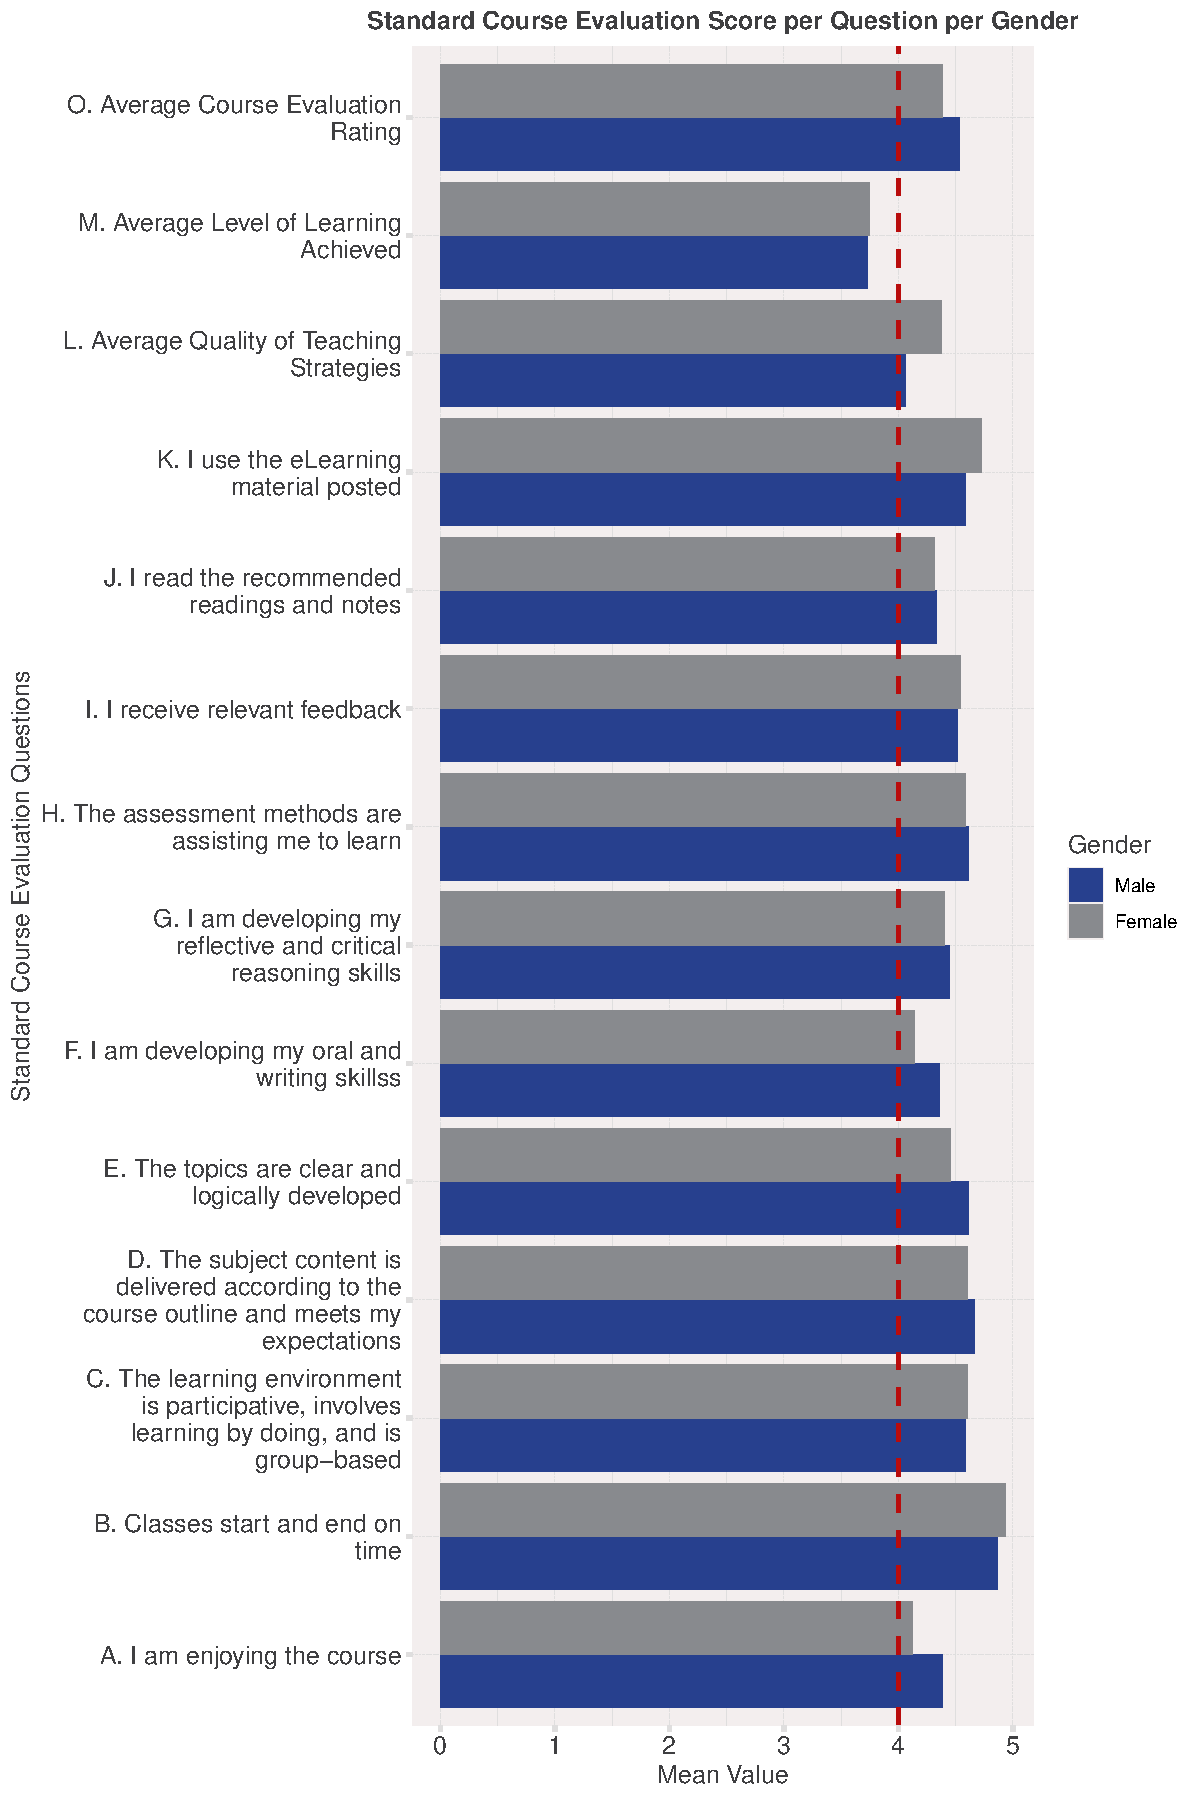
\includegraphics{Mid-SemesterCourseEvaluation-20240819-20241125-ADB-BBIT2.2_files/figure-latex/VisualizationsForCourseEvaluationResultsperGender-1.pdf}

\newpage

The \textbf{``Average Course Evaluation Rating''} variable in the plot
below indicates the score \textbf{per class group} with a baseline of
4/5.

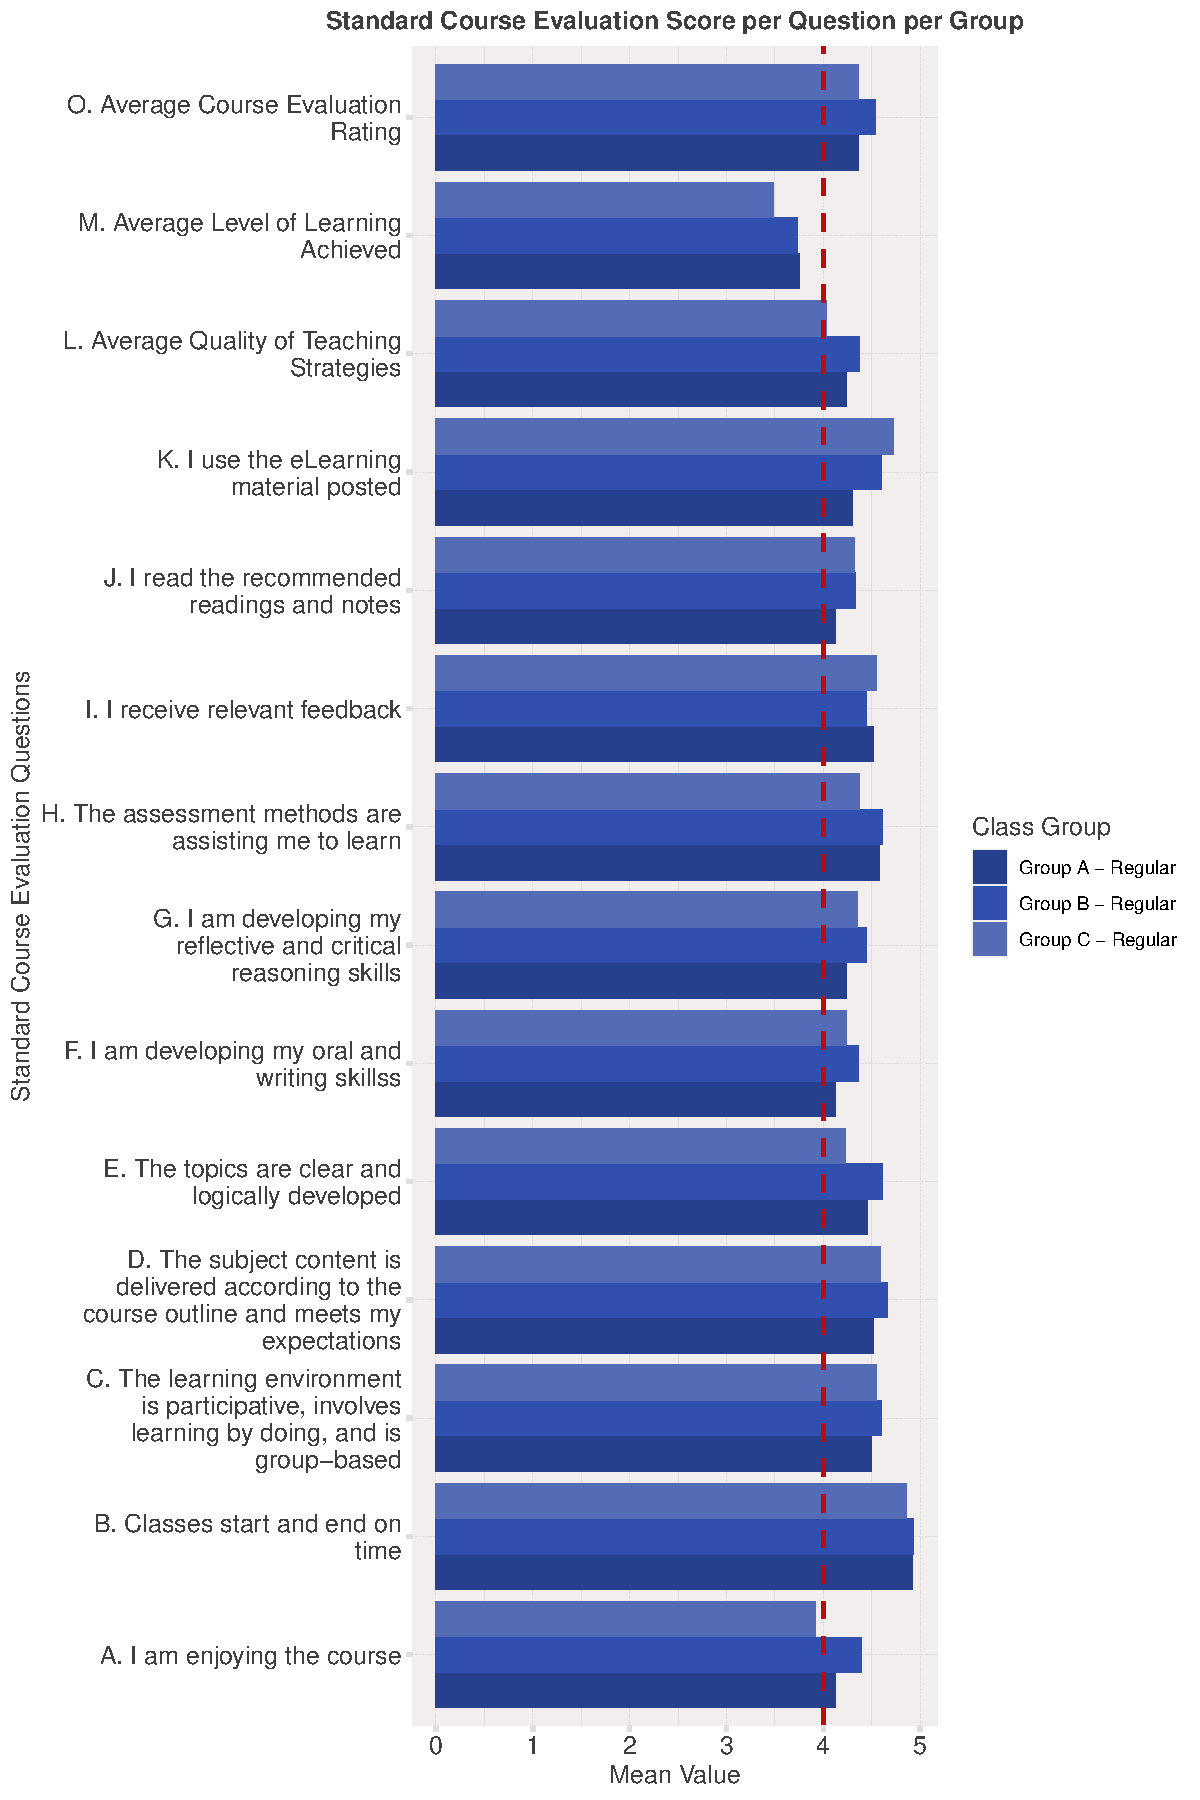
\includegraphics{Mid-SemesterCourseEvaluation-20240819-20241125-ADB-BBIT2.2_files/figure-latex/VisualizationsForCourseEvaluationResultsperGroup-1.pdf}

\newpage

\subsection{Correlations}\label{correlations}

The specific correlation values are presented below:

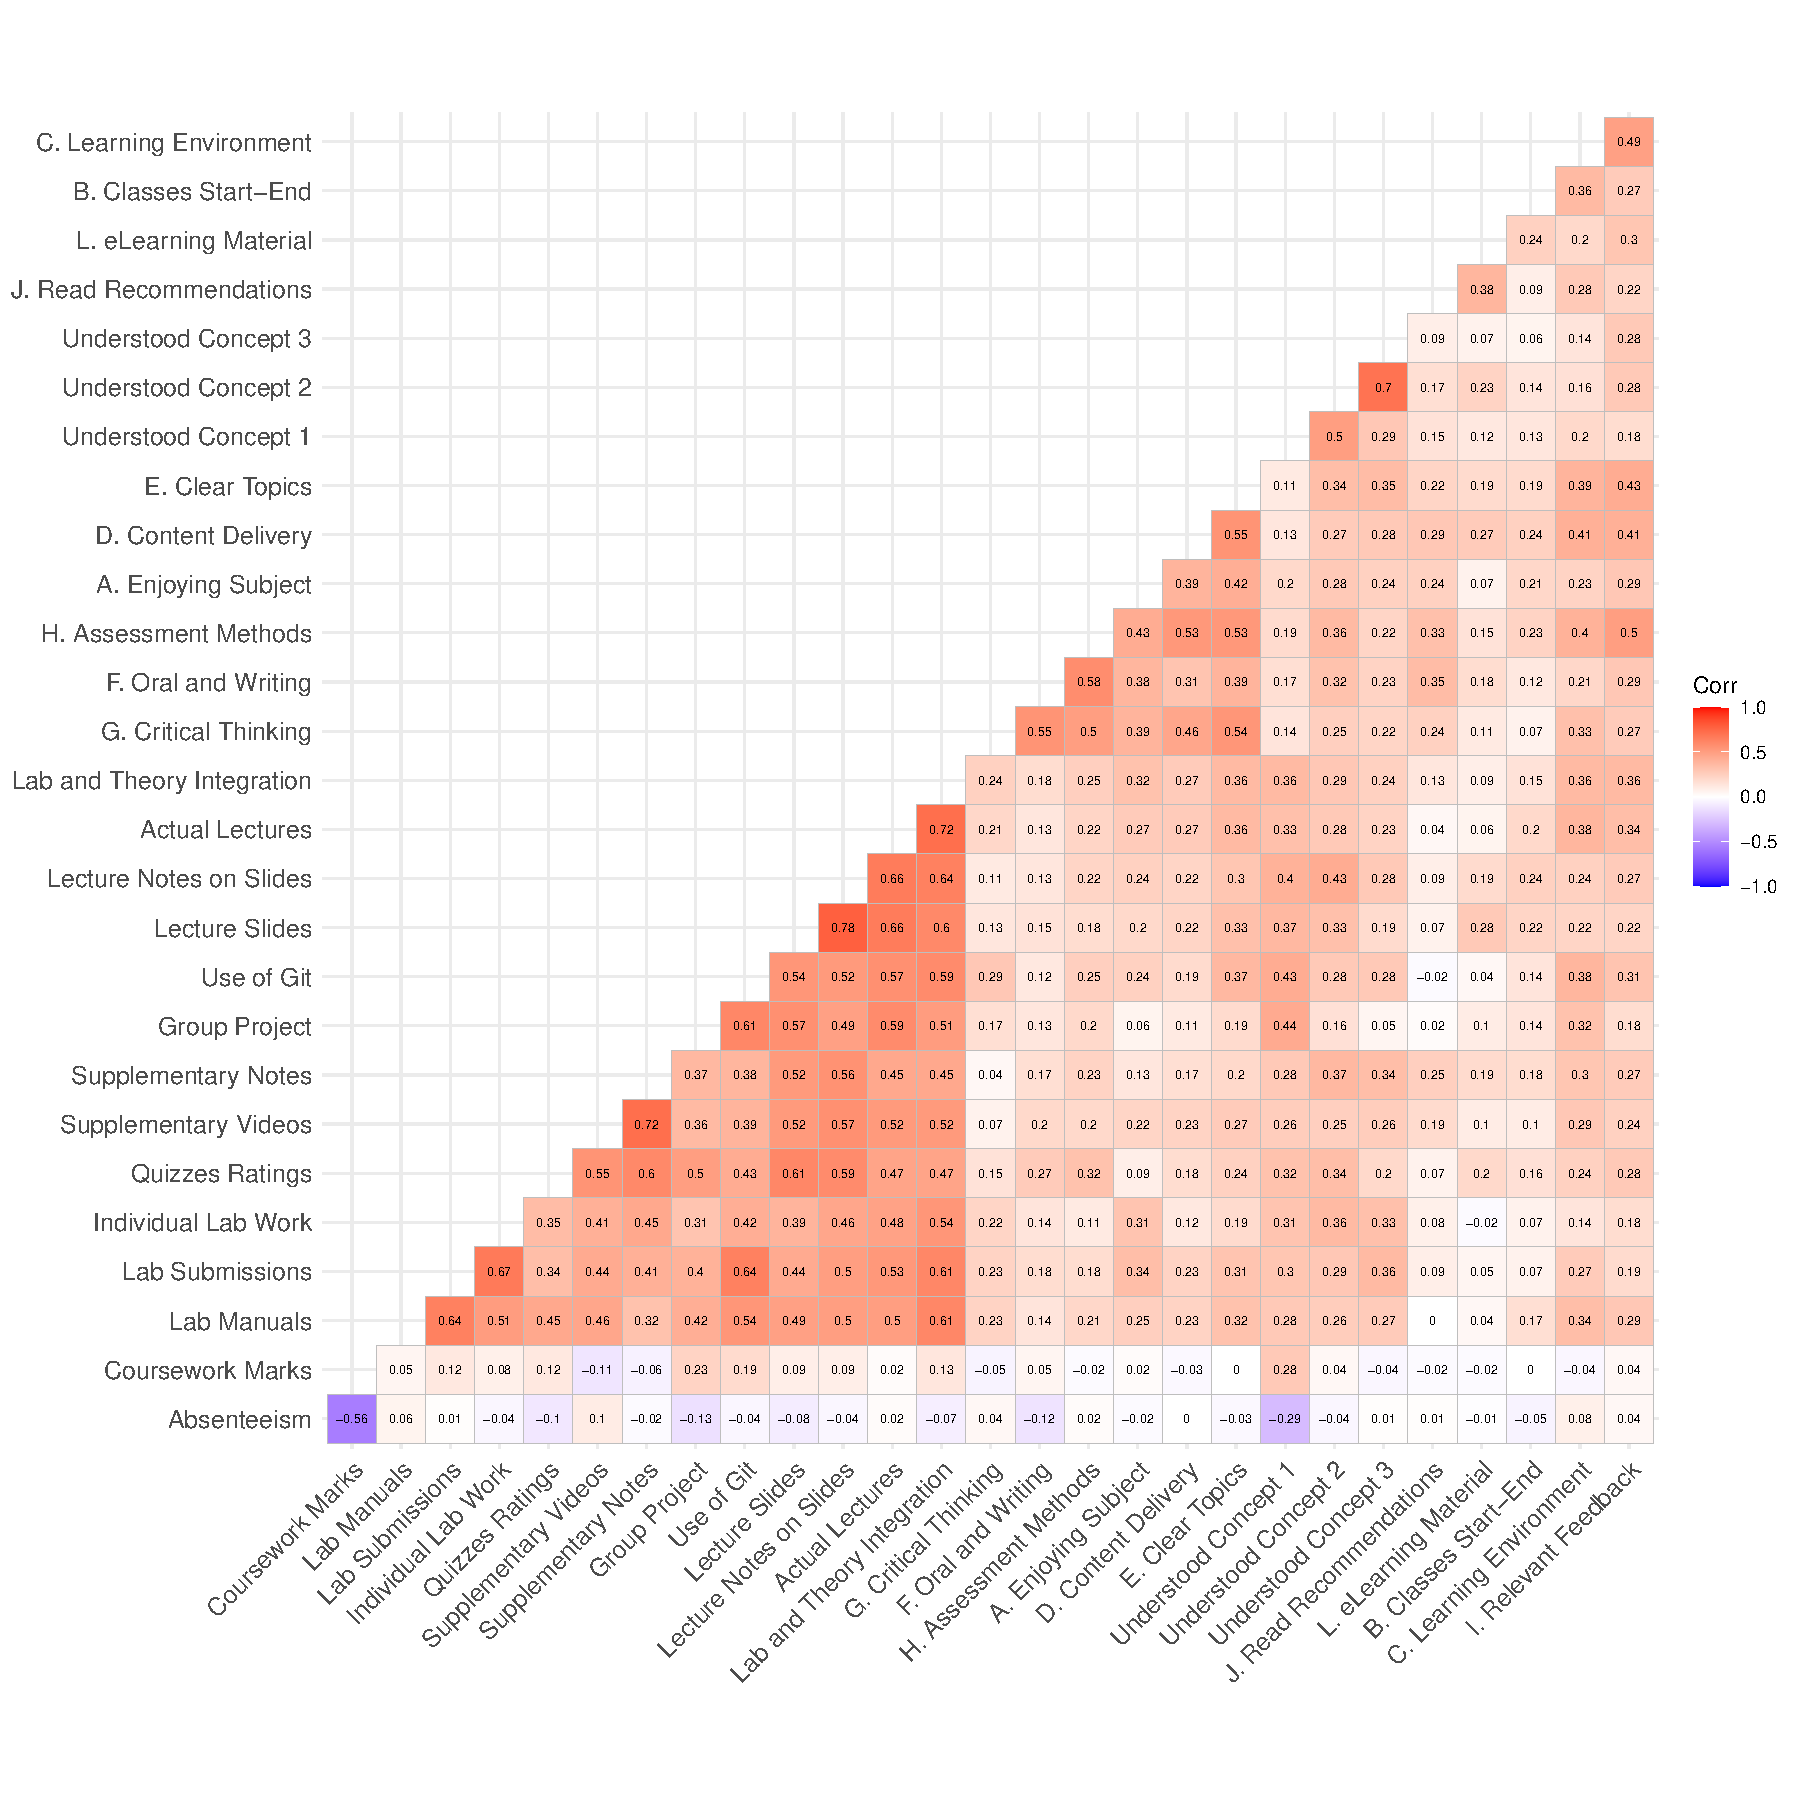
\includegraphics{Mid-SemesterCourseEvaluation-20240819-20241125-ADB-BBIT2.2_files/figure-latex/CorrelationMatrixWithFigures-1.pdf}

\subsubsection{Interesting Correlations}\label{interesting-correlations}

Correlations worth noting include:

\begin{itemize}
\item
  \textbf{0.78 correlation} between ``lectures slides'' and ``lecture
  notes on some of the lecture slides'': \emph{Having lecture notes to
  accompany some lecture slides improves the overall quality of the
  lecture slide}
\item
  \textbf{0.72 correlation} between ``Supplementary videos to watch as
  an additional explanation of a topic'' and ``Supplementary content to
  read'': \emph{Students who find the supplementary videos useful with
  regad to their learning also find the supplementary notes useful}
\item
  \textbf{0.72 correlation} between ``the quality of the lectures given
  (quality measured by the breadth (the full span of knowledge of a
  subject) and depth (the extent to which specific topics are focused
  upon, amplified, and explored) of learning - NOT quality measured by
  how fun, comical, or entertaining the lectures are)'' and ``the
  integration of practical labs in most classes even if it is not in a
  computer lab'': \emph{Mixing practicals with theory in the same class
  improves the overall quality of the lecture.}
\item
  \textbf{0.7 correlation} between ``understood Concept 2 (Conceptual
  Data Modelling)'' and ``understood Concept 3 (Database Constraints)'':
  \emph{Students who do not understand Concept 2 also do not understand
  Concept 3. It is necessary to understand Concept 2 before moving on to
  Concept 3.}
\item
  \textbf{-0.56 correlation} between ``Absenteeism'' and ``Coursework
  Marks'': \emph{The higher the absenteeism, the lower the student's
  coursework marks}
\item
  \textbf{-0.29 correlation} between ``Absenteeism'' and ``Understood
  Concept 1'': \emph{The more late students are to register for the
  course, the harder it is for them to understand concept 1}
\end{itemize}

\newpage

The negative correlation between ``absenteeism'' and ``coursework
marks'' is stronger among the female students, i.e., the more classes a
student misses, the worse their performance, especially for female
students.

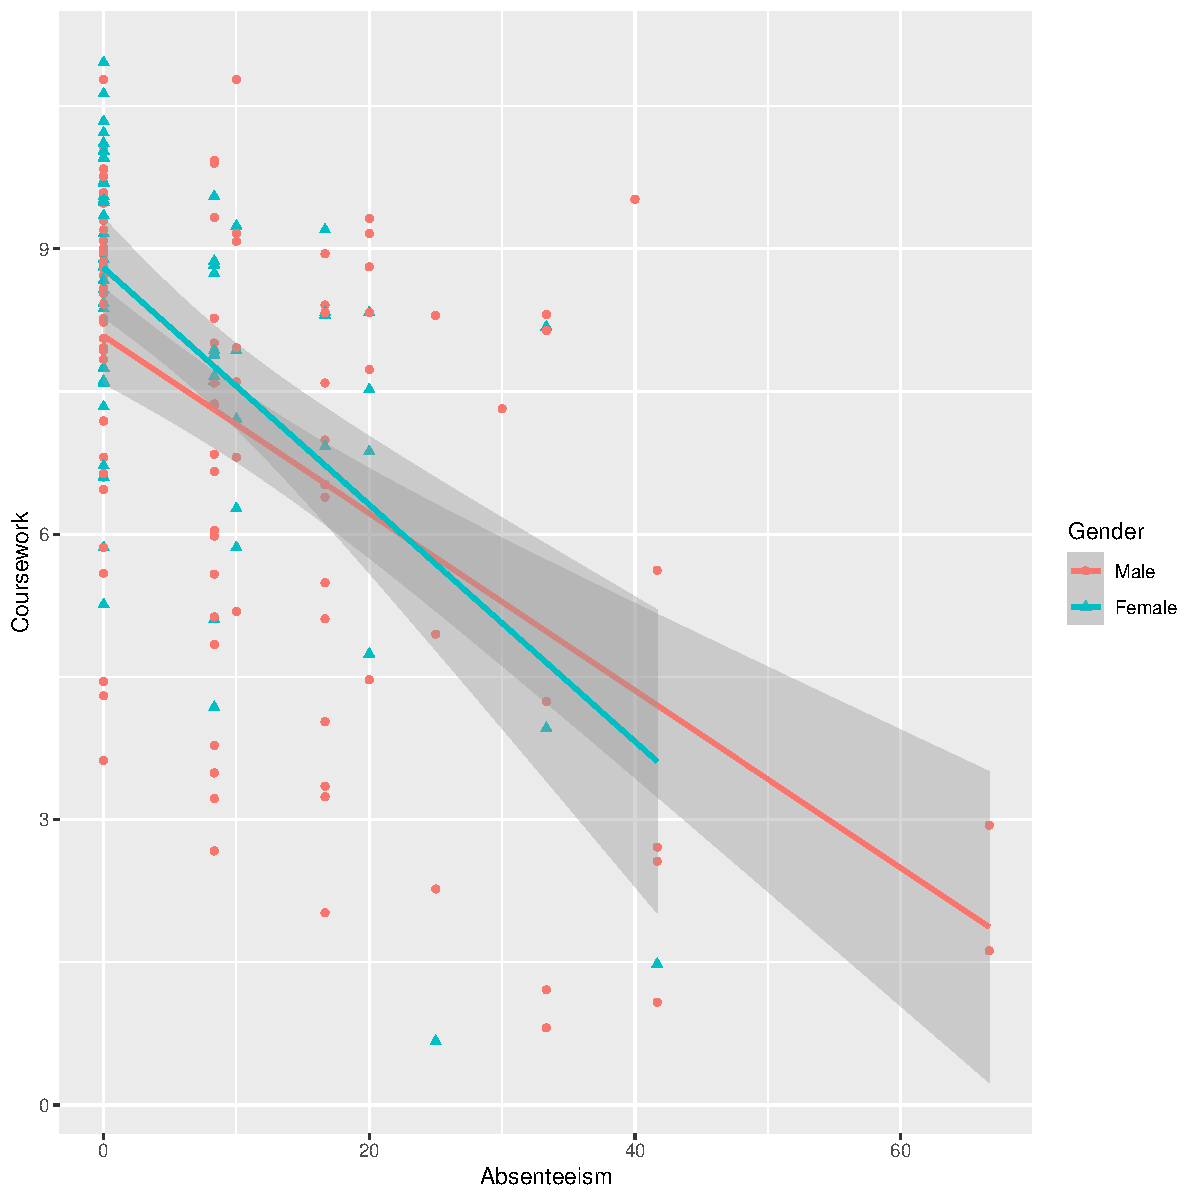
\includegraphics{Mid-SemesterCourseEvaluation-20240819-20241125-ADB-BBIT2.2_files/figure-latex/DrillDownCorr1-1.pdf}

\newpage

\subsubsection{Absenteeism Percentage}\label{absenteeism-percentage}

\paragraph{Absenteeism by Specific Class
Group}\label{absenteeism-by-specific-class-group}

Group C has the lowest absenteeism issues despite having a class on
Friday afternoon.

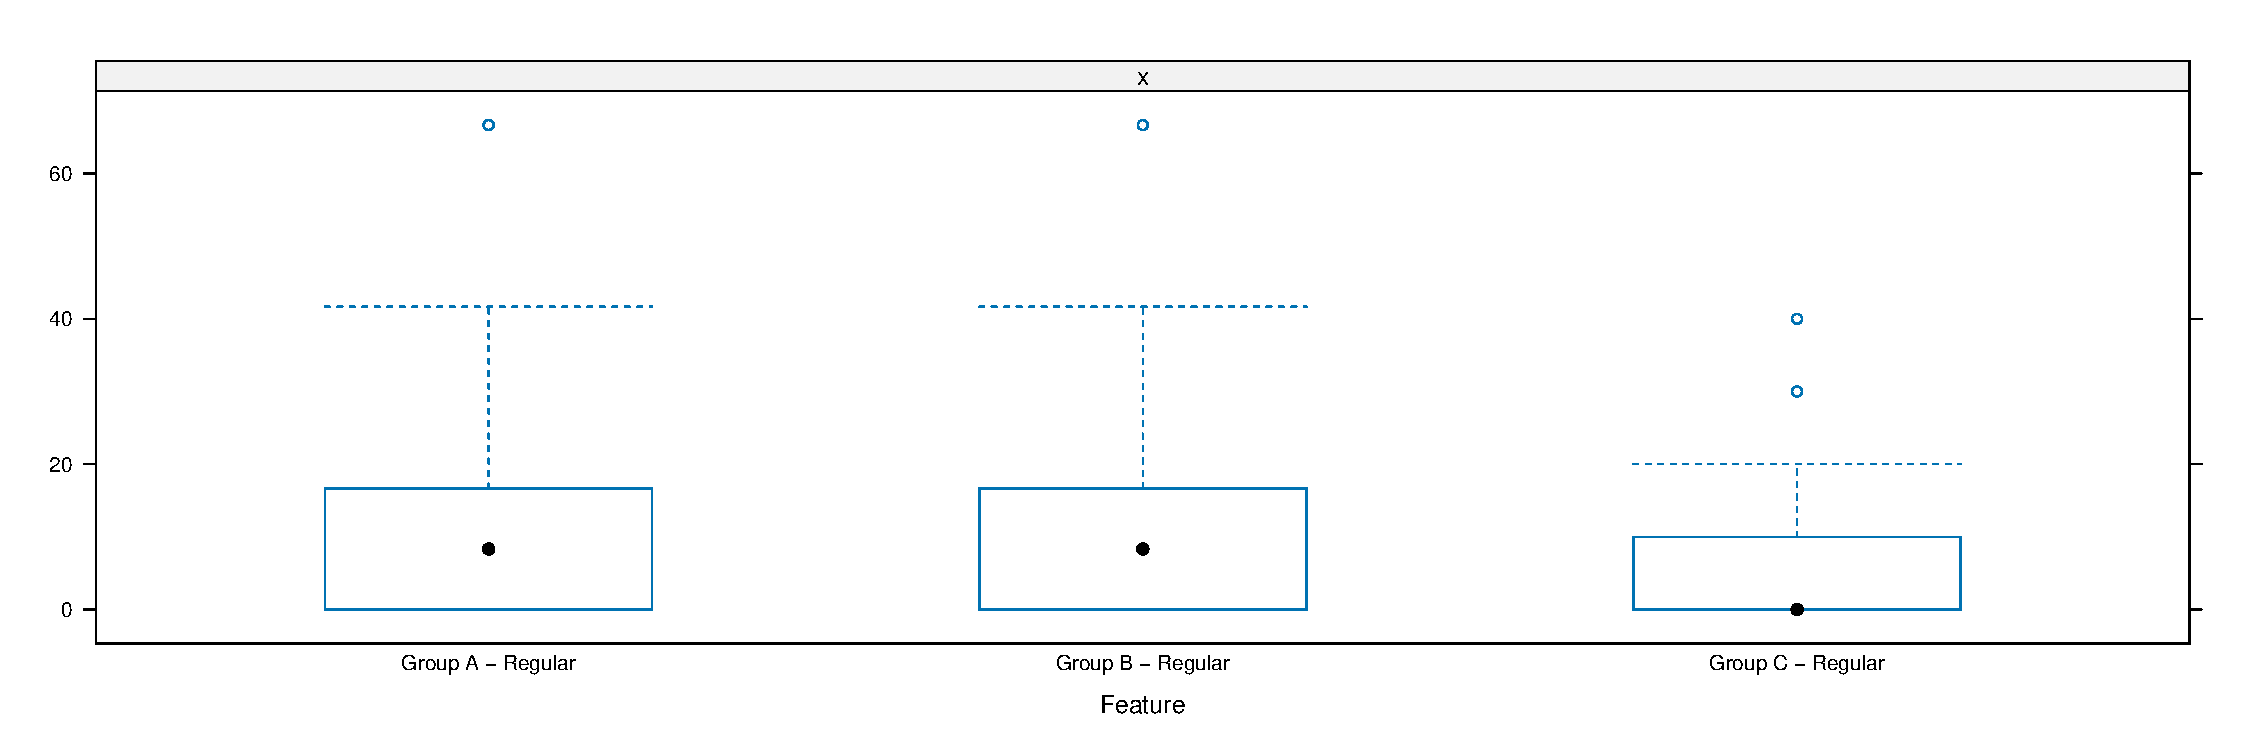
\includegraphics{Mid-SemesterCourseEvaluation-20240819-20241125-ADB-BBIT2.2_files/figure-latex/AbsenteeismBoxandWhiskerSpecificGroup-1.pdf}

\paragraph{Absenteeism by Gender}\label{absenteeism-by-gender}

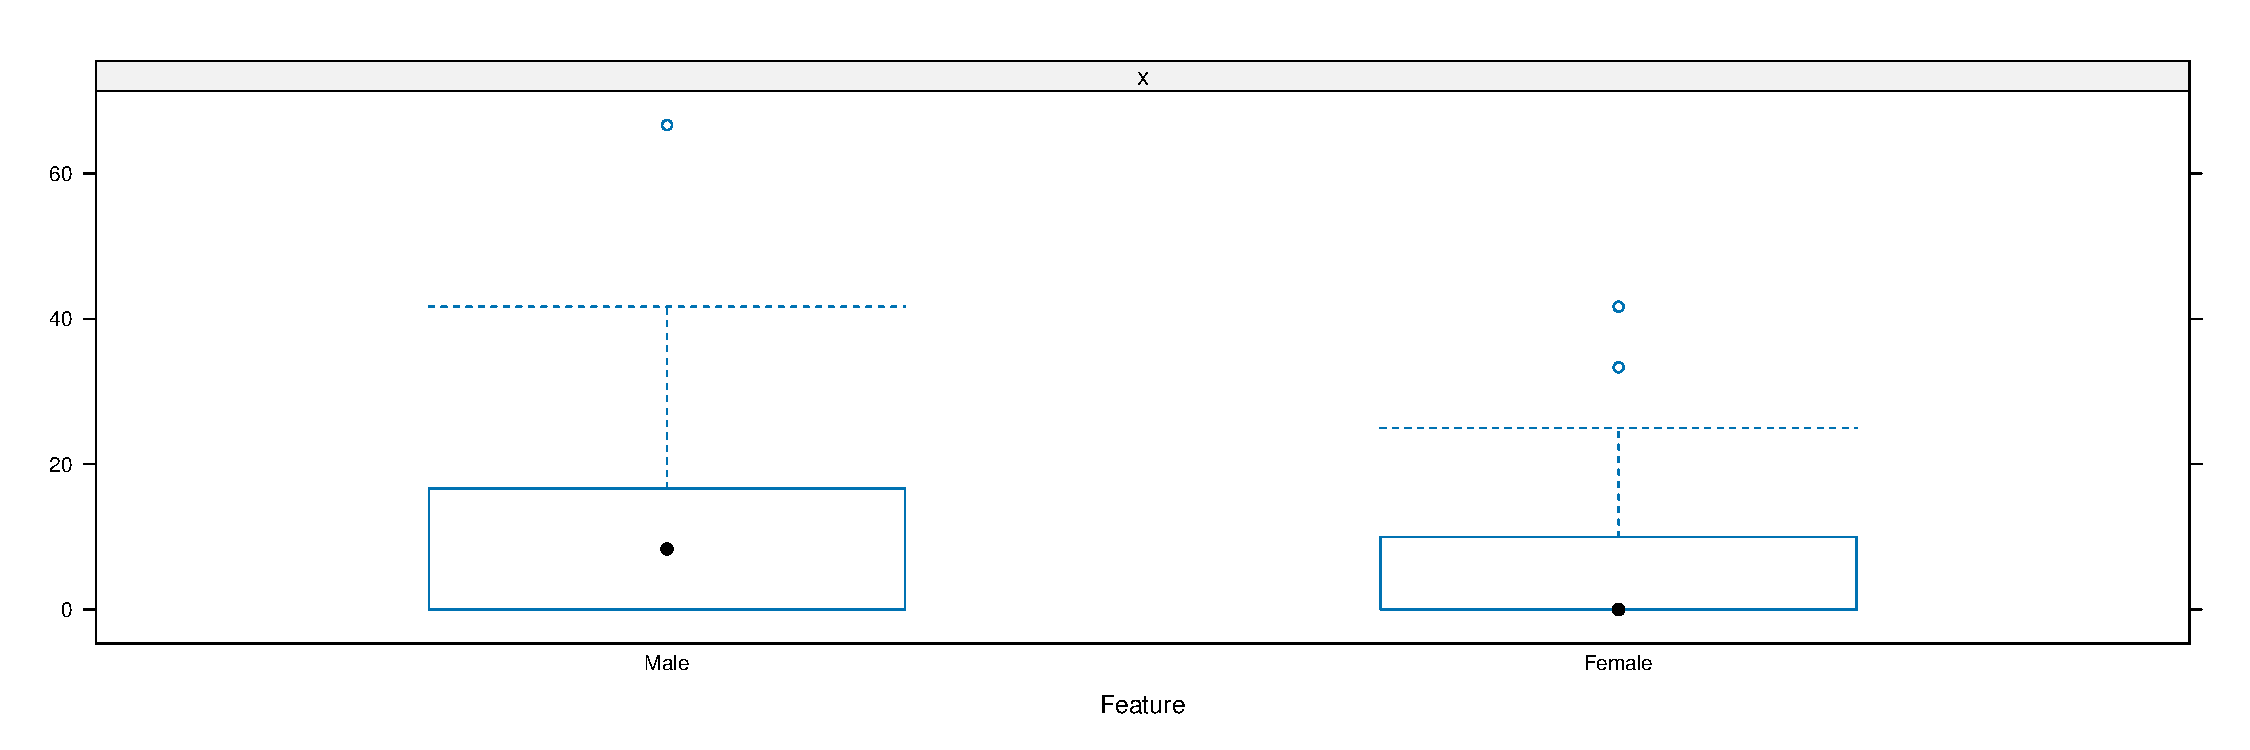
\includegraphics{Mid-SemesterCourseEvaluation-20240819-20241125-ADB-BBIT2.2_files/figure-latex/AbsenteeismBoxandWhiskerGender-1.pdf}

\newpage

\section{Qualitative Data Analysis}\label{qualitative-data-analysis}

\subsection{Sentiment Analysis
(Lexicon-Based)}\label{sentiment-analysis-lexicon-based}

The ``likes'' refer to the answer to the question, ``Write at least two
things you like about the teaching and learning in this unit so far.''
The sentiments expressed through the ``likes'' are:

The ``wishes'' refer to the answer to the question, ``Write at least one
recommendation to improve the teaching and learning in this unit (for
the remaining weeks in the semester)''. The sentiments expressed through
the ``wishes'' are:

\newpage

\subsubsection{Chord Diagram of Sentiments for Likes per Class
Group}\label{chord-diagram-of-sentiments-for-likes-per-class-group}

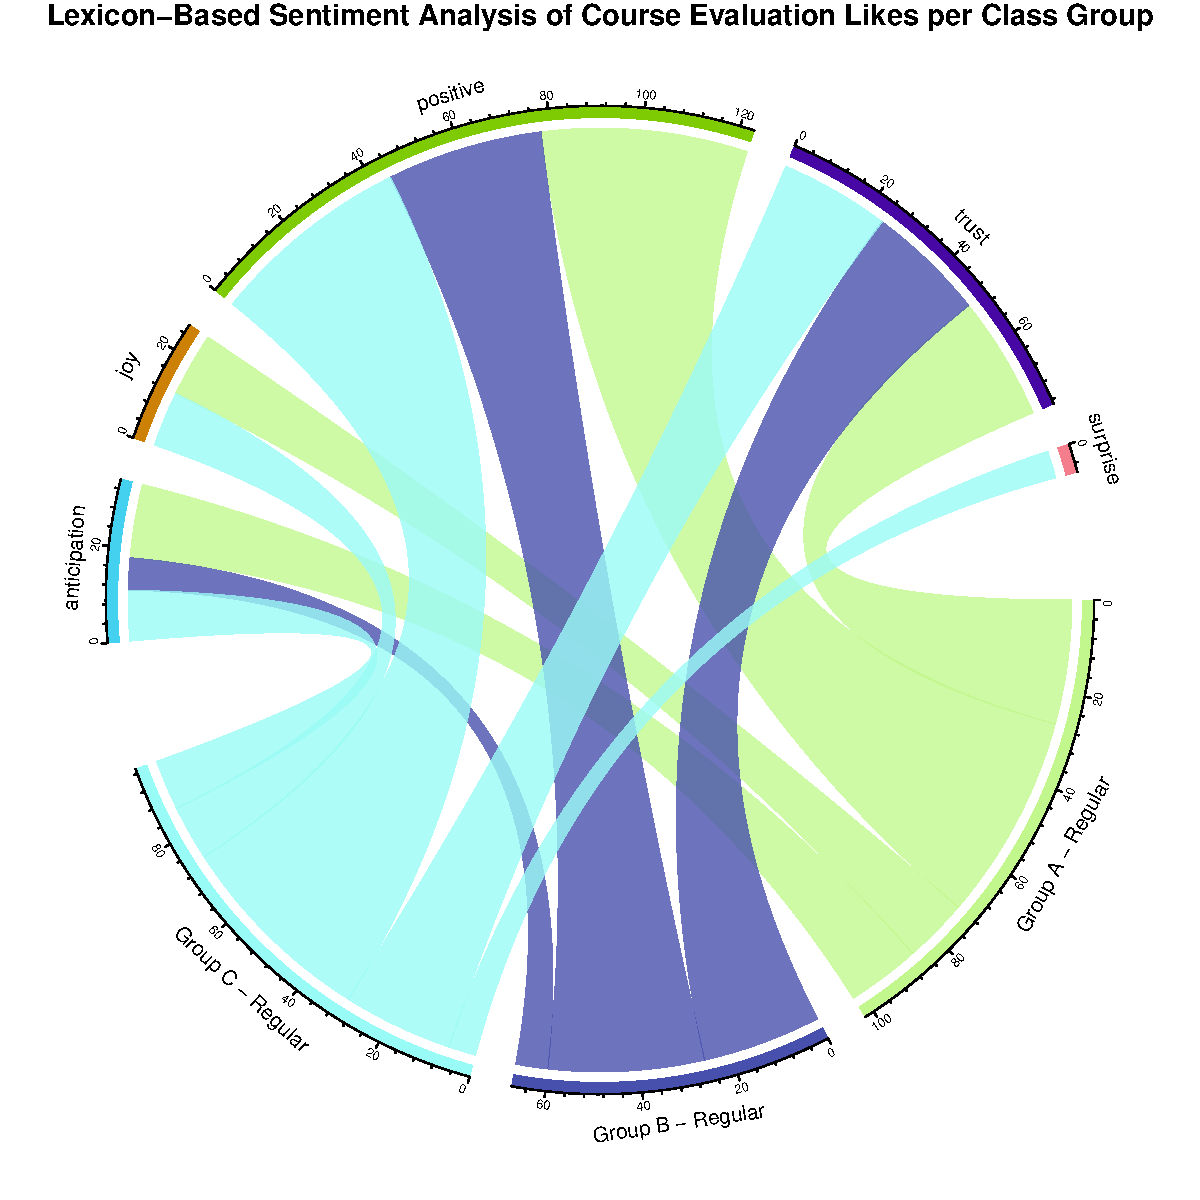
\includegraphics{Mid-SemesterCourseEvaluation-20240819-20241125-ADB-BBIT2.2_files/figure-latex/ChordDiagramLikesPerGroup-1.pdf}

\newpage

\subsubsection{Chord Diagram of Sentiments for Likes per Class
Gender}\label{chord-diagram-of-sentiments-for-likes-per-class-gender}

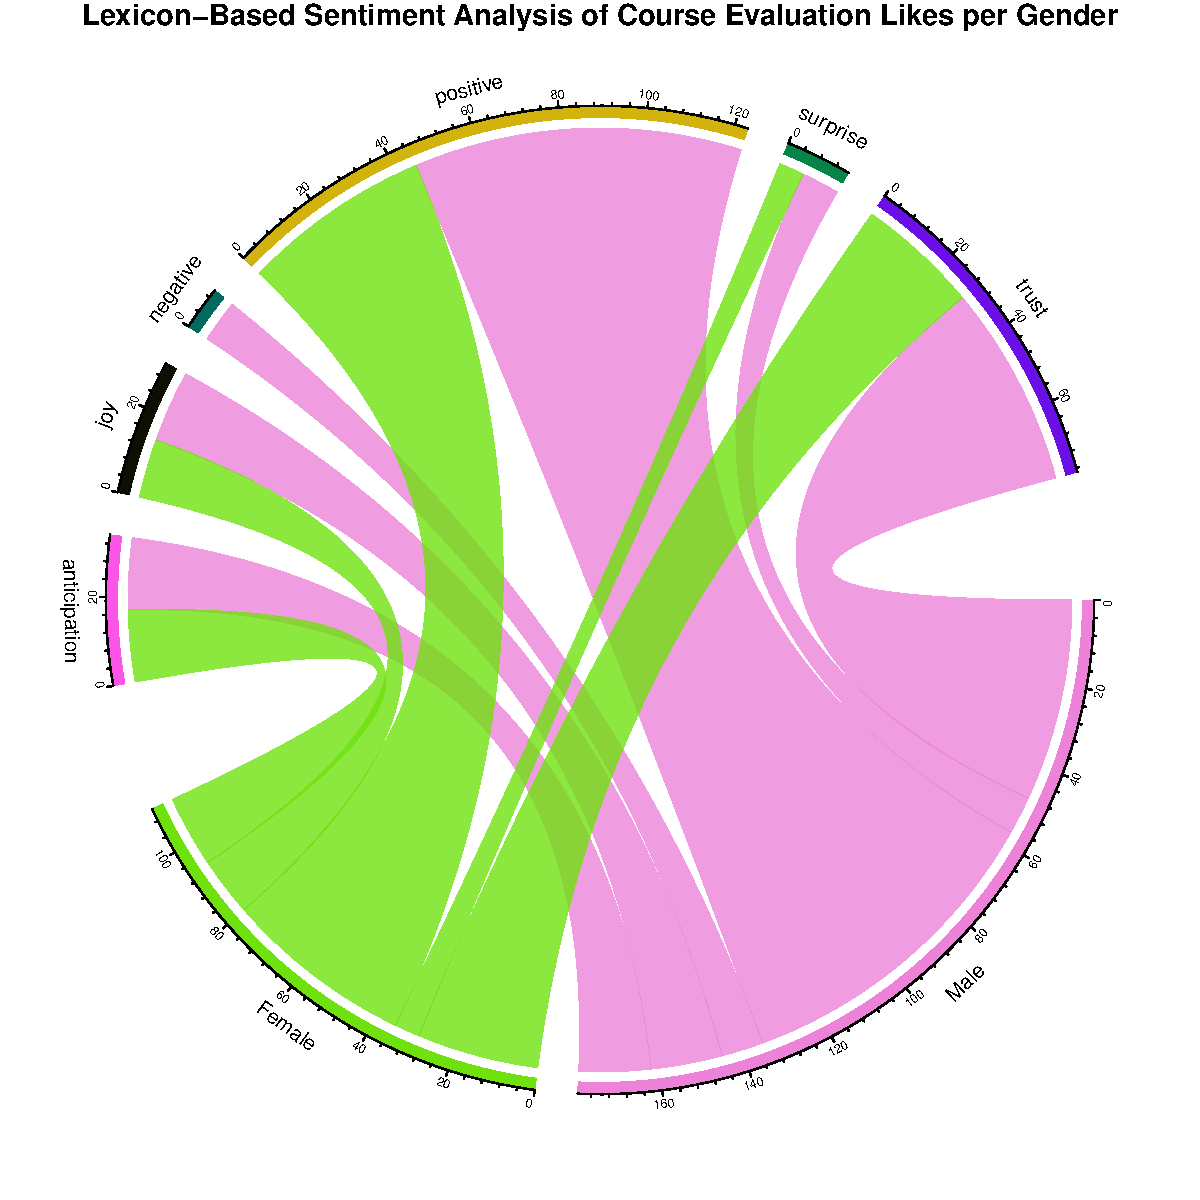
\includegraphics{Mid-SemesterCourseEvaluation-20240819-20241125-ADB-BBIT2.2_files/figure-latex/ChordDiagramLikesPerGender-1.pdf}

The results are similar for both genders but the male students are more
positive and trustworthy based on their choice of words for the ``likes
question''.

\newpage

\subsubsection{Chord Diagram of Sentiments for Wishes per Class
Group}\label{chord-diagram-of-sentiments-for-wishes-per-class-group}

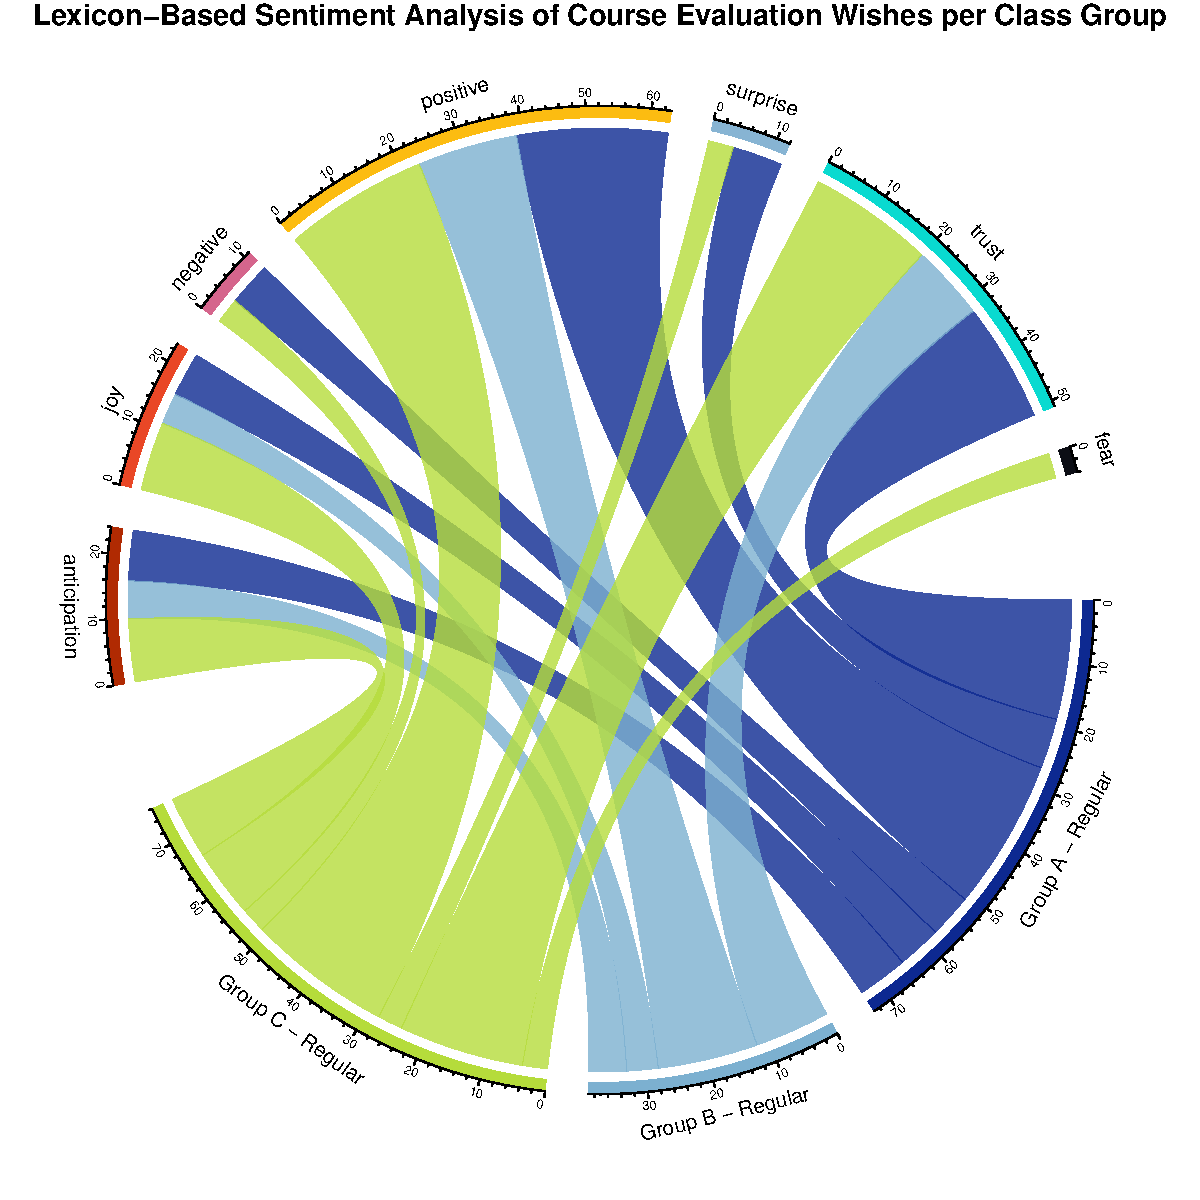
\includegraphics{Mid-SemesterCourseEvaluation-20240819-20241125-ADB-BBIT2.2_files/figure-latex/ChordDiagramPerGroup_Wishes-1.pdf}

Group A and C express more negative sentiments with Group C also
expressing fear based on their choice of words for the ``wishes
question''.

\newpage

\subsubsection{Chord Diagram of Sentiments for Wishes per
Gender}\label{chord-diagram-of-sentiments-for-wishes-per-gender}

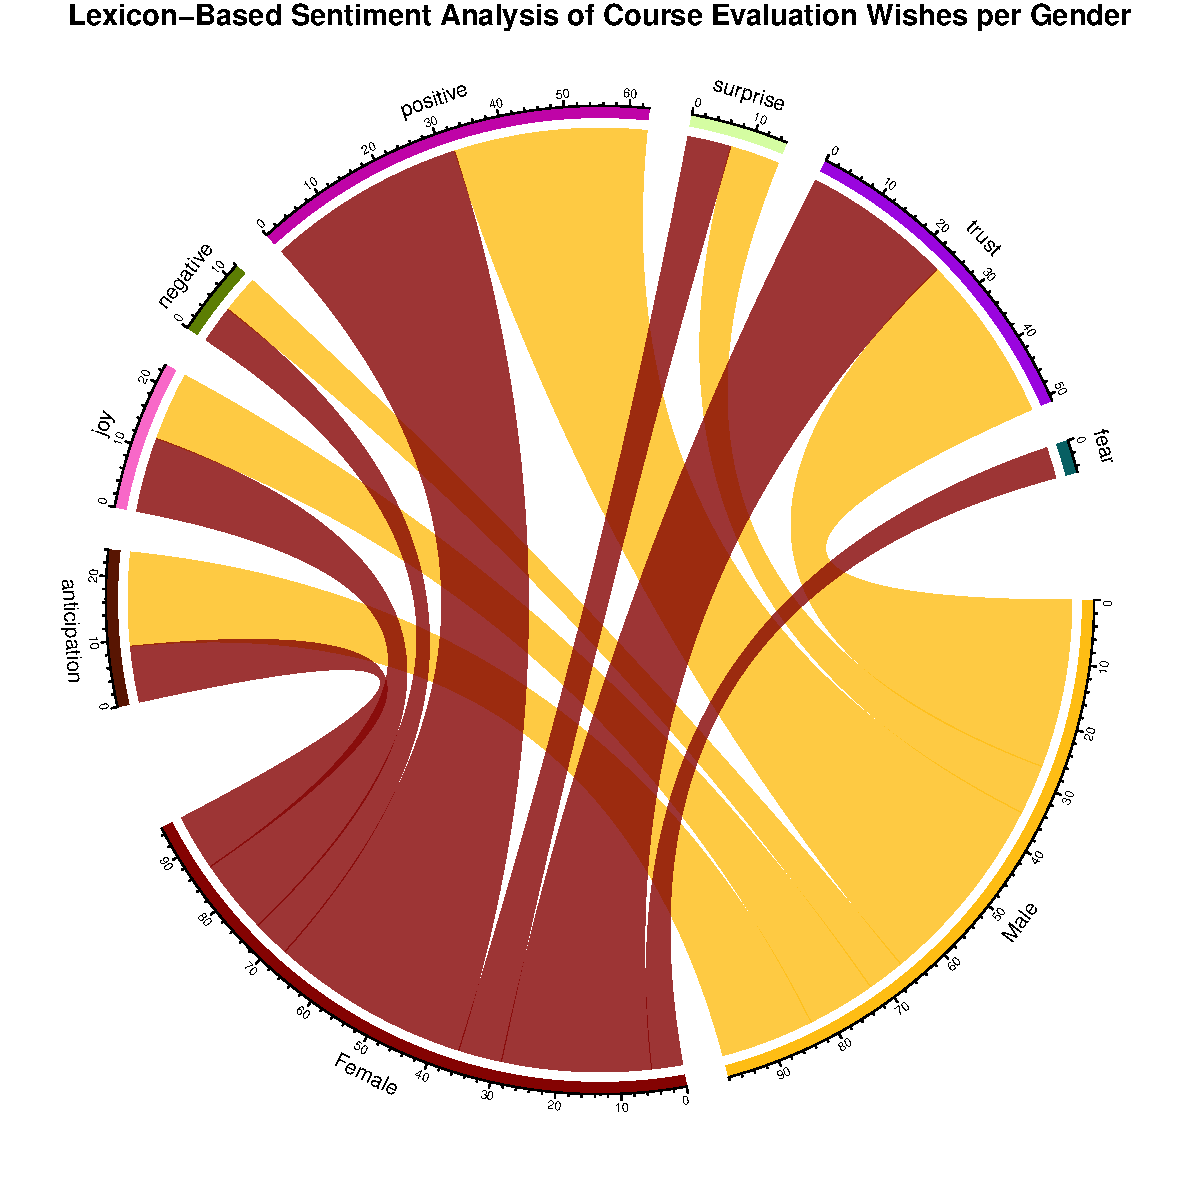
\includegraphics{Mid-SemesterCourseEvaluation-20240819-20241125-ADB-BBIT2.2_files/figure-latex/ChordDiagramPerGender_Wishes-1.pdf}

The sentiments for wishes are similar across both genders but female
students express more fear than male students based on their choice of
words.

\newpage

\subsection{Topic Modelling (Latent Dirichlet Allocation (LDA)
based)}\label{topic-modelling-latent-dirichlet-allocation-lda-based}

The goal of topic modelling is to identify latent (hidden) terms
(topics) in the students' course evaluation textual feedback. In this
case, a topic is a mixture of words and a student's textual feedback is
a combination of one or more topics (mixed-membership model).

The 2 topics for the ``likes'' (as guided by the LDA model) are:

\begin{enumerate}
\def\labelenumi{\arabic{enumi}.}
\item
  Topic 1: Well-Taught for Ease of Understanding
\item
  Topic 2: Practical
\item
  Topic 3: Organized
\end{enumerate}

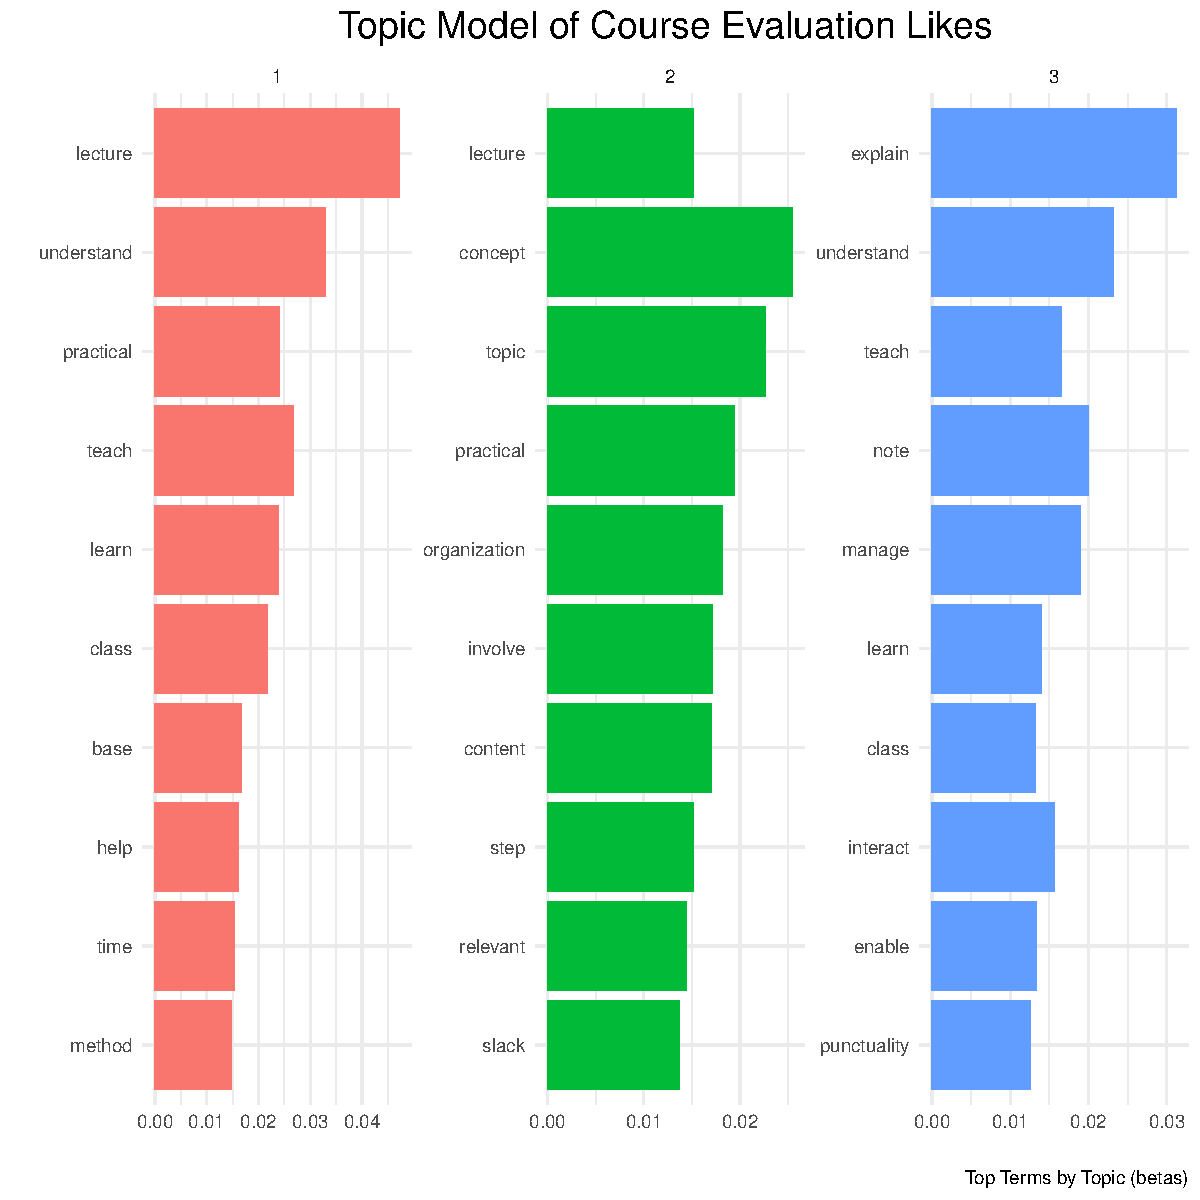
\includegraphics{Mid-SemesterCourseEvaluation-20240819-20241125-ADB-BBIT2.2_files/figure-latex/visualizations_for_likes_topic_modelling-1.pdf}

\newpage

The 5 topics for the ``wishes'' (as guided by the LDA model) are:

\begin{enumerate}
\def\labelenumi{\arabic{enumi}.}
\item
  Topic 1: Extend the deadlines
\item
  Topic 2: Reduce the group work
\item
  Topic 3: More breaks during lectures
\end{enumerate}

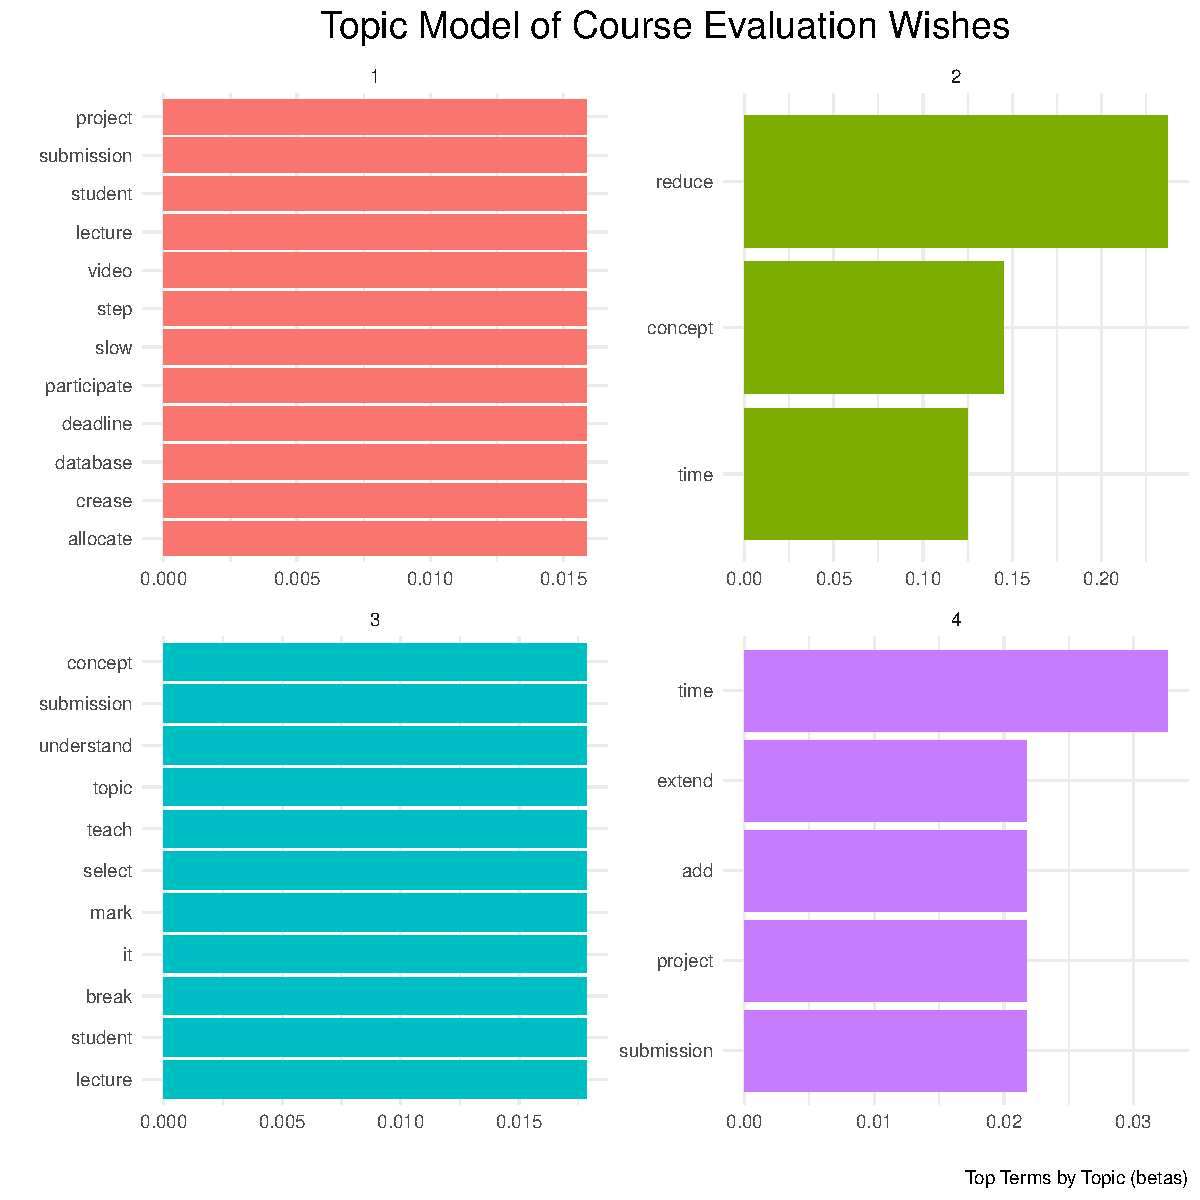
\includegraphics{Mid-SemesterCourseEvaluation-20240819-20241125-ADB-BBIT2.2_files/figure-latex/visualizations_for_wishes_topic_modelling-1.pdf}

\newpage

\section{Appendices}\label{appendices}

\subsection{Appendix A: Full Name of
Variables}\label{appendix-a-full-name-of-variables}

The following variables have been renamed to fit the correlation plots:

\begin{verbatim}
`A. Enjoying Subject` = `B - 1. I am enjoying the course`,
`B. Classes Start-End` = `B - 2. Classes start and end on time`,
`C. Learning Environment` = `B - 3. The learning environment is participative, involves learning by doing, and is group-based`,
`D. Content Delivery` = `B - 4. The subject content is delivered according to the course outline and meets my expectations`,
`E. Clear Topics` = `B - 5. The topics are clear and logically developed`,
 `F. Oral and Writing` = `B - 6. I am developing my oral and writing skills`,
`G. Critical Thinking` = `B - 7. I am developing my reflective and critical reasoning skills`,
 `H. Assessment Methods` = `B - 8. The assessment methods are assisting me to learn`,
`I. Relevant Feedback` = `B - 9. I receive relevant feedback`,
`J. Read Recommendations` = `B - 10. I read the recommended readings and notes`,
`L. eLearning Material` = `B - 11. I use the eLearning material posted`,
`Understood Concept 1` = `C - 1. Concept 1 of 6: Business Processes`,
`Understood Concept 2` = `C - 2. Concept 2 of 6: Conceptual Data Modelling`,
`Understood Concept 3` = `C - 3. Concept 3 of 6: Database Constraints`,
# `Acquired Skill 1` = `Q04_Competency for Technologies->D - 1. ChartJS`,
# `Acquired Skill 2` = `Q04_Competency for Technologies->D - 2. R (includes R markdown and R plumber)`,
# `Acquired Skill 3` = `Q04_Competency for Technologies->D - 3. MySQL`,
# `Acquired Skill 4` = `Q04_Competency for Technologies->D - 4. Kafka`,

# `Acquired Skill 5` = `Q04_Competency for Technologies->D - 5. ksqlDB`,
# `Acquired Skill 6` = `Q04_Competency for Technologies->D - 6. ClickHouse`,
# `Acquired Skill 7` = `Q04_Competency for Technologies->D - 7. Linear and Non-Linear ML Algorithms in the caret package`,

`Group Project` = `D - 1. The group project`,
`Quizzes Ratings` = `D - 2. Quizzes at the end of each concept`,
`Lab Manuals` = `D - 3. Lab manuals that outline the steps to follow during the labs`,
`Lab Submissions` = `D - 4. Required lab work submissions at the end of each lab manual that outline the activity to be done on your own`,
`Use of Git` = `D - 5. Labs that require you to use Git to work in a team`,
`Individual Lab Work` = `D - 6. Labs that require you to work alone`,
`Supplementary Videos` = `D - 7. Supplementary videos to watch as an additional explanation of a topic`,
`Supplementary Notes` = `D - 8. Supplementary content to read`,
`Lecture Slides` = `D - 9. Lectures slides`,
`Lecture Notes on Slides` = `D - 10. Lecture notes on some of the lecture slides`,
`Actual Lectures` = `D - 11. The quality of the lectures given (quality measured by the breadth (the full span of knowledge of a subject) and depth (the extent to which specific topics are focused upon, amplified, and explored) of learning - NOT quality measured by how fun, comical, or entertaining the lectures are)`,
`Lab and Theory Integration` = `D - 12. The integration of practical labs in most classes even if it is not in a computer lab`,
`Coursework Marks` = `Coursework`
\end{verbatim}

\newpage

\subsection{Appendix B: Raw Qualitative
Data}\label{appendix-b-raw-qualitative-data}

\subsubsection{Likes}\label{likes}

The raw data of the likes is as follows:

.begin\{longtable\}{[}t{]}\{\textgreater\{

\raggedright

\arraybackslash\}p\{35em\}\}

\caption{\label{tab:RawLikesData}Write two things you like about the teaching and learning in this unit so far}

\textbackslash{} \toprule Comment (Likes)\textbackslash{} \midrule Class
punctuality Community feedback on Slack\textbackslash{} \hline I love
that we have labs that enable me to engage with the content and get some
experience of what I would be needed to do in the work
environment.\textbackslash{} \hline N/A\textbackslash{} \hline The
content delivery is well done\textbackslash{} \hline -\textbackslash{}
\hline I like the learning pace and the content with the labs is
executable\textbackslash{} \hline The topics Labs and group
work\textbackslash{} \hline The delivery The \vphantom{2}
content\textbackslash{} \hline The quizzes, how we learned to use new
software i.e.~Slack\textbackslash{} \hline Inclusive learning relevant
feedback is given\textbackslash{} \hline Coding in vs and applying it in
GitHub\textbackslash{} \hline None\textbackslash{} \hline
n/a\textbackslash{} \hline Null\textbackslash{} \hline I like how we are
given a quiz after each concept in this unit. In this unit, I also like
the way we already have all the content online for the whole
semester.\textbackslash{} \hline The learning is very enjoyable and
interesting\textbackslash{} \hline I like the concept of doing the short
quizzes on google classroom\textbackslash{} \hline Triggers and also
capabilities and constraints\textbackslash{} \hline Lessons are
interesting and push us to get more knowledge and to do
better\textbackslash{} \hline It is Fun. It is
interactive\textbackslash{} \hline
1. I enjoy how organized the results are so I am able to track my
performance from the start to the finish 2. I like how detailed the lab
manuals are because I am able to fully understand what is
happening\textbackslash{} \hline its interesting. its
relevant\textbackslash{} \hline I like that it is much more practical as
performing activities is much more beneficial that just sitting an
having the information exposited, I also like that the steps for the
practicals are detailed and give explanations on their
functions\textbackslash{} \hline I like that the lecturer gives feedback
regarding the projects and labs and that the classes start on
time\textbackslash{} \hline The lecturer has great delivery method and
tries to be at per with his class The lecturer takes his work seriously
and gives his students clear expectations\textbackslash{} \hline The
class is quite interactive and teamwork is also shown in
class\textbackslash{} \hline the quizes given the way the content is
delivered\textbackslash{} \hline I like how informative the unit is. I
like how there is time allocated to work with my peers, it allows me to
understand the concepts more.\textbackslash{} \hline The lecturer
explains things well,the lec goes with a good pace\textbackslash{}
\hline configuration of a database transaction event
scheduling\textbackslash{} \hline Its interactive\textbackslash{} \hline
interactiveness and time keeping\textbackslash{} \hline Assistance when
someone has issues during labworks The step by step procedures to do the
labs\textbackslash{} \hline Broading my knowledge and
unnderstanding\textbackslash{} \hline 1.The quizzes 2.The
project\textbackslash{} \hline The timely response on slack The quizzes
after each concept\textbackslash{} \hline The delivery of the
content,the lecturer's commitment on assisting a peson
individually\textbackslash{} \hline \#NAME?\textbackslash{} \hline
\#NAME?\textbackslash{} \hline the topics are taught well , One is
guided and what and how they are supposed to do the
exercises\textbackslash{} \hline OK\textbackslash{} \hline
1. The lecturer takes his time to explain concepts 2. The lab
manuals.are well laid out\textbackslash{} \hline The quiz The
project\textbackslash{} \hline topic one and two\textbackslash{} \hline
The group work makes it fun and engaging The lecturer manages time well,
classes end in good time\textbackslash{} \hline The group project The
way everything is organized\textbackslash{} \hline Its good that you
keep pushing us \ldots. Thats what amazes me in this
unit\textbackslash{} \hline Content delivery Quizes\textbackslash{}
\hline It is very organized, the assignments, labs and group work The
concepts are understandable\textbackslash{} \hline Explaining being
explained in steps by the lecturer.\textbackslash{} \hline Learning new
things. We do most of the work ourselves so we learn while
practicing\textbackslash{} \hline Lecturer explains everything to the
tea\textbackslash{} \hline .\textbackslash{} \hline The lecturer is
always punctual The learning is efficient\textbackslash{} \hline
Lecturer\textbackslash{} \hline Fun\textbackslash{} \hline
1. I like it 2.Good lectures\textbackslash{} \hline It is very
interactive and fun I get to learn new skills based on different
perspectives\textbackslash{} \hline 1.Very well explained
2.Interesting\textbackslash{} \hline It is very practical Feedback is
relevant and on time\textbackslash{} \hline The practicals The
teamwork\textbackslash{} \hline the detailed explained slides and the
time taken to make sure everyone understands\textbackslash{} \hline The
unit is really involving which is good The unit is
interesting\textbackslash{} \hline The clear outline of the work The
practical examples\textbackslash{} \hline The applicability of the unit
in modern world\textbackslash{} \hline I like the labs and quizzes which
check on our progress\textbackslash{} \hline I like how the lecturer
explains the concepts clearly and logically I like the fact that the lec
is always ready to explain unclear and ambiguous
concepts\textbackslash{} \hline Well Organised,
Interactive\textbackslash{} \hline The lecturer and what is being
taught\textbackslash{} \hline Use of real world examples. And Use of
structured design and logical thinking\textbackslash{} \hline Learning
new skills Learning problem solving\textbackslash{} \hline Practice is
very important for the long run, Database is very broad\textbackslash{}
\hline The explanation is simple and easy for me to understand. The
class is involving by asking questions\textbackslash{} \hline it is
mostly practical\textbackslash{} \hline the lab exercises are engaging
if one is committed to them.

the extensive use of the GitHub repositories and the other database
tools are equipping with practical database experiences\textbackslash{}
\hline Simple\textbackslash{} \hline -\textbackslash{} \hline i.)
Classes start and end on time ii.) Lab practiclals are interractive and
are fun to do\textbackslash{} \hline The topics are well explained and
to one's understanding and learning the topics are interesting as
compared to labs\textbackslash{} \hline I like the clarity that is
offered and the avaliability of the lecturer\textbackslash{} \hline He
is very organised He is patient when it comes to
explaining\textbackslash{} \hline simplified mode of teaching proper
organization of content\textbackslash{} \hline
1. Well organized work plan 2. Good amount of work load
given\textbackslash{} \hline It is very practical and well
detailed\textbackslash{} \hline the quizzes that are given out after
each concept are really helpful\textbackslash{} \hline Everything is
well outlined and oranised he explains the concepts in a good
way\textbackslash{} \hline How the lecturer organises his work so its
easy to find the material that you need\textbackslash{} \hline The
practical interaction with the content The methods of checking content
retention\textbackslash{} \hline The organisation of the lecturers
materials The feedback given and the ability to track
progress\textbackslash{} \hline It is giving me more ideas and knowledge
It is helping in my oral skills\textbackslash{} \hline The way the
concept is taught with like the examples that are
understandable\textbackslash{} \hline The quizes offered really help in
summarising the topic The lab work manual is simple and easy to
follow\textbackslash{} \hline The group work given by the lecturer helps
in my understanding of the concept better The quizzes done after every
concept which helps me in reminding myself on the
concept\textbackslash{} \hline
1. The lecturer is very organized and teaches the content well. 2.
Resources and materials required to take on this unit are readily
available.\textbackslash{} \hline The group gave me idea on how to apply
the concepts in real life\textbackslash{} \hline The hands-on
practicals. The lab manuals.\textbackslash{} \hline I like the
lecturere\ldots He is wonderful and fair\textbackslash{} \hline I like
the practical aspect of the unit I like how we explore different aspects
of the database\textbackslash{} \hline
1. I enjoy the content and lectures in general 2. I like the labs and
the manuals are helpful for understanding\textbackslash{} \hline the
ability to engage in critical thinking and group
participation\textbackslash{} \hline group work and the
quizes\textbackslash{} \hline The teacher know how to explain the theory
parts\textbackslash{} \hline I like the amount of group work that we're
given because during the undertaking of the work, I get to learn new
concepts. Watching supplementary videos online. Some of the videos
explain the content in a simpler way.\textbackslash{} \hline Topics well
developed Able to ask questions freely\textbackslash{} \hline The
lecturer's teaching style is interactive\textbackslash{} \hline It is
well explained Lecture tutors well\textbackslash{} \hline We are first
taught then we do practically which is really helpful The lecturer
responds to those who have not understood.He takes time to teach certain
concepts\textbackslash{} \hline It's engaging and the lab works make it
much more interesting. In the few past weeks, I've learned a lot more
than I learned in the past semester.\textbackslash{} \hline Helps in
thinking critically about data management. Additionally the
collaborative projects foster teamwork and problem solving
skills.\textbackslash{} \hline The group work\textbackslash{} \hline I
like the organization\textbackslash{} \hline Mode of
delivery,\textbackslash{} \hline It's good\textbackslash{} \hline It's
engaging It is practical hence keeping you on your toes\textbackslash{}
\hline I am able to solve real world problems I am able to logically
think\textbackslash{} \hline \#NAME?\textbackslash{} \hline The lecturer
ensures that he has expounded on the topic of the day The lecturer asks
questions that engage the class\textbackslash{} \hline The lecturer
explains the concepts in detail before the lab exercises. The lecturer
is ready to help whenever a challenge arises when doing the lab manuals
in class.\textbackslash{} \hline The group work concept The lecture is
always ready to explain a concept you've not understood\textbackslash{}
\hline
1. The teaching methods the lecture always make sure that every student
has understood.2. The learning environment .\textbackslash{} \hline I'm
enjoying the unit so far\textbackslash{} \hline The lab works are
educative and creates innovativion\textbackslash{} \hline how it is
interactive the group work\textbackslash{} \hline It is very practical
so it really helps with hands on skills Content is clearly broken down
and understandable\textbackslash{} \hline the topics are well detailed,
explanation is well given\textbackslash{} \hline It is mostly
practical.\textbackslash{} \hline It requires me to be more active and
keen\textbackslash{} \hline The lec The \vphantom{1}
content\textbackslash{} \hline very interesting\textbackslash{} \hline
Many quizzes help understand\textbackslash{} \hline The notes are
comprehensive and the methods of evaluation are
effective\textbackslash{} \hline practically done\textbackslash{} \hline
1: It has group based activities. 2: Some business concepts are
involved.\textbackslash{} \hline Teaching methods Venue\textbackslash{}
\hline Classes start and end on time\textbackslash{} \hline Well
organized, clear explanations\textbackslash{} \hline 1.Good lectures
2.Friendly lecturer\textbackslash{} \hline The Lecturer is
considerate(available for consultation and what not)\textbackslash{}
\hline The lecturer involves students in answering questions during
lectures which keeps them attentive The lectures are light and easy to
understand making them enjoyable\textbackslash{} \hline The quizzes at
the end of each concept help me to remember things The group work is
really helpful\textbackslash{} \hline
1. It is easy to understand. 2. It enables me to earn more marks in
coursework.\textbackslash{} \hline course delivery materials and the
lecturer is organized\textbackslash{} \hline I like how time is
kept\textbackslash{} \hline Good feedback Step by step
guidelines\textbackslash{} \hline Punctuality of the
lecturer\textbackslash{} \hline interactive learning experience notes
are clear\textbackslash{} \hline Use of groups Use of
quizes\textbackslash{} \hline The concept\textbackslash{} \hline It is
interactive and knowledge based\textbackslash{} \hline The concept of
containerization and using of docker and Dbeaver\textbackslash{} \hline
ive learnt how to run diffrent containers on dbeaver as well on my
vscode ranging from python, php e.t.c\textbackslash{} \hline Time
management, punctuality\textbackslash{} \hline Quiz after every
concept\textbackslash{} \hline I like the way that like deliver the
contents and gives us a lot of labs\textbackslash{} \hline The hands-on
approach in this unit, especially with using tools like MySQL and
Docker, has been really beneficial. I appreciate the collaborative
aspect of this unit, especially through GitHub and other group
assignments.\textbackslash{} \hline I like the involving labwork I like
how groupwork enables me to learn from my friends\textbackslash{} \hline
It is more practical than theoretical The fact that we have all the
topics before class\textbackslash{} \hline The content\textbackslash{}
\hline The quiz after every major topic\textbackslash{} \hline Notes are
provided and the quizes are helpful\textbackslash{} \hline I like how we
have quizzes at the end of each session and also the way the teacher is
always available\textbackslash{} \hline The group work on github and
also class and the quizzes after class\textbackslash{} \hline I like the
mode of teaching the lecturer offers, he is well organized and orderly
in the way he presents his materials and notes in class\textbackslash{}
\hline fun\textbackslash{} \hline I like that the lecturer is on point
and brief and the group based assignments\textbackslash{} \hline The
teacher is very intentional. The knowledge acquired is very
deep.\textbackslash{} \hline Time management and reading
materials\textbackslash{} \hline The lecturer is easy to reach The
lecturer is willing to help\textbackslash{} \hline containerization
concept\textbackslash{} \hline i like the method of teaching the
lecturere is good and calm\textbackslash{} \hline The teacher is very
responsive The unit is delivered at the students pace\textbackslash{}
\bottomrule \textbackslash end\{longtable\}

\newpage

\subsubsection{Wishes}\label{wishes}

The raw data of the wishes is as follows:

.begin\{longtable\}{[}t{]}\{\textgreater\{

\raggedright

\arraybackslash\}p\{35em\}\}
\textbackslash caption\{\label{tab:RawWishesData}Write at least one
recommendation to improve the teaching and learning in this unit (for
the remaining weeks in the semester).\textbackslash{} \toprule Comment
(Wishes)\textbackslash{} \midrule None\textbackslash{} \hline Extend
deadlines for labs.\textbackslash{} \hline N/A\textbackslash{} \hline
More code explanation\textbackslash{} \hline Lab manuals are nit
straight forward\textbackslash{} \hline To allow quizzes to be done
outside class time\textbackslash{} \hline Introduce breaks in between
the lessons\textbackslash{} \hline Be a bit flexible on the lab
submissions to enable catching up\textbackslash{} \hline In addition to
the quizzes we have, more quizzes that don't have an impact on
coursework\textbackslash{} \hline More group related
working\textbackslash{} \hline N/A\textbackslash{} \hline
None\textbackslash{} \hline recommend you slow down the pace of teaching
and please be more engaging with the class\textbackslash{} \hline
Null\textbackslash{} \hline The lecturer should share with us more
online resources, mostly videos, to help us easily and quickly
internalize some of the complex concepts.\textbackslash{} \hline To
repeat what we have learnt previously\textbackslash{} \hline Easier
labs\textbackslash{} \hline more deadline on lab
submissions\textbackslash{} \hline After every topic we hope to get at
least a summary of if\textbackslash{} \hline Added time to do lab
work\textbackslash{} \hline N/A\textbackslash{} \hline teaching more
theory\textbackslash{} \hline I wish the balance between group and
individual work was better as there is way more group work than
individual and i personally learn best myself\textbackslash{} \hline The
lecturer could introduce breaks in the middle of the
class\textbackslash{} \hline reduced group work\textbackslash{} \hline
Requesting the lecturer to be sending us like reference videos which we
can use to like expand froma what he has taught or like a video that can
help one understnd more on what he has taught\textbackslash{} \hline to
slow down abit\textbackslash{} \hline To reduce the speed at which some
of the concepts are covered.\textbackslash{} \hline making sure everyone
is not left behind\textbackslash{} \hline I would recommend that you
show us why and how they are applied in real-life by giving out real
based examples or one of your projects as an example just to help us
know how they are implemented.\textbackslash{} \hline More
quizes\textbackslash{} \hline More time on labs\textbackslash{} \hline
Having reasonable submission time, given the hefty timetable this
semester.\textbackslash{} \hline Be clear on the topics being tested and
consider we have other units other than this one so we have enough
time\textbackslash{} \hline 1.Group work should be marked according to
the work done by each member seeing as there some members don't
participate in group work 2. Could we also have a break mid
lesson\textbackslash{} \hline More labs to emphasize in the different
concepts\textbackslash{} \hline More time should be allocated to finish
up the quizes and the projects\textbackslash{} \hline Lecturer to go at
a moderate speed\textbackslash{} \hline \#NAME?\textbackslash{} \hline
Keep updating the knowledge\textbackslash{} \hline Give us
breaks.\textbackslash{} \hline Adequate time for lab
submissions\textbackslash{} \hline More quiz\textbackslash{} \hline the
lab lecture slides\textbackslash{} \hline I am content\textbackslash{}
\hline Review of quizzes and labs\textbackslash{} \hline Yes pushing us
is good but it would be better if we go a bit slowly\textbackslash{}
\hline More quizzes A deeper explanation on lab manuals\textbackslash{}
\hline more revisions\textbackslash{} \hline Increasing deadlines for
submitting the lab works.\textbackslash{} \hline Explain things in an
easier way to understand\textbackslash{} \hline More fun
engagement\textbackslash{} \hline Allocate more time for the lab
assignments\textbackslash{} \hline Everything is okay\textbackslash{}
\hline Less work\textbackslash{} \hline clear \vphantom{1}
notes\textbackslash{} \hline more time for submission\textbackslash{}
\hline We should engage more with the lecturer\textbackslash{} \hline
Extended duration of time for lab manuals group work\textbackslash{}
\hline The unit is fine for me. I am content with everything the
lecturer has done so far to make our life studying this unit
easier\textbackslash{} \hline Class participation\textbackslash{} \hline
I recommend maybe re evaluating the quizzes as already it's a lot to
handle with labs we do and the documentation, considering we also have
other units it proves difficult to always be at par with
you.\textbackslash{} \hline The class should be made more
lively\textbackslash{} \hline .\textbackslash{} \hline Lab time
submittion should be extended\textbackslash{} \hline i think its going
okay\textbackslash{} \hline A little bit more time on labs
deadline\textbackslash{} \hline N/A\textbackslash{} \hline More time
added to submission time for work\textbackslash{} \hline Peer
review\textbackslash{} \hline None\textbackslash{} \hline
N/A\textbackslash{} \hline Remind us the relevant concepts of Database 1
and not assume that we know\textbackslash{} \hline some more time for
the labs\textbackslash{} \hline emphasis on ensuring students are clear
about the course outline and the amount of commitment it requires before
hand\textbackslash{} \hline Timing\textbackslash{} \hline
-\textbackslash{} \hline To carry out lab practicals with students
during class so we can easily identify errors together and move as one
unit.\textbackslash{} \hline Explain the lab processes much better and
slower for one to understand\textbackslash{} \hline More group
presentations\textbackslash{} \hline The lecturers tone. To project his
voice abit more.\textbackslash{} \hline The lecturer should add us more
time to work on the projects and labs since there is a lot to be covered
but the time is too short The lecturer should not assume that we know
certain things mostly during the labs\textbackslash{} \hline More
individual exercises\textbackslash{} \hline I would request that the
labs be doen if possible at a slower pace\textbackslash{} \hline time
allocated for the project should be increased\textbackslash{} \hline
Extending the lab submission times Better elaboration on the
labs\textbackslash{} \hline As he marks the labs, he should include
comments on what about your work is outstanding or
missing\textbackslash{} \hline Grading criteria sharing\textbackslash{}
\hline More recaps on some concepts of the database 1 Recaps on the
material where we did by ourselves to understand the reasoning behind
the grade\textbackslash{} \hline Give us time to finish the lab
works\textbackslash{} \hline Explain better how the lab work and the
projects are intergrated it's a bit confusing\textbackslash{} \hline
give us more time to finish the labs\textbackslash{} \hline The
engagement of the lecturer\textbackslash{} \hline Find a way to make
sure each group member participates and not just get carried by other
group members as well as measures to ensure each student is on board
with what is happening and not lost.\textbackslash{} \hline To give us
more time for the lab work\textbackslash{} \hline Reduced group
work\textbackslash{} \hline A better way for helping those left behind
with the labs\textbackslash{} \hline Some of the steps in the Lab rarely
execute correctly. Can you kindly once in a while go through the lab
step by step\textbackslash{} \hline I would prefer if we could do the
labs individually since working in groups is a little stressful and one
person mostly does the work (in my experience) however I understand if
that would not be possible\textbackslash{} \hline engagement in group
work\textbackslash{} \hline more group presentations\textbackslash{}
\hline A better follow up on the lab manuals\textbackslash{} \hline More
recommendations on the youtube videos\textbackslash{} \hline Moving at a
moderate pace rather than fast pace\textbackslash{} \hline Extended time
frame to submit project and labs\textbackslash{} \hline Lecturer explain
better on lab works\textbackslash{} \hline Kindly give us enough time to
do the group work .. not teaching on Friday and work is due the next
day\textbackslash{} \hline I wish we learn more about transactions. And
also how to deployments of databases/containers.\textbackslash{} \hline
Allow us to be able to correct our labs\textbackslash{} \hline Same time
as the other groups to complete our work. We usually get less
time\textbackslash{} \hline Not to rush to finish the syllabus take time
to make sure we (the students)we understand\textbackslash{} \hline
Increase of assessment deadlines\textbackslash{} \hline Give atleast 3-4
days for the lab work\textbackslash{} \hline To go slow on the labs
since one can easily be left behind\textbackslash{} \hline Maybe adding
case studies to the learning process\textbackslash{} \hline I have no
recommendations. The learning and teaching methods are
satisfactory\textbackslash{} \hline More topical quizzes\textbackslash{}
\hline Kindly extend the deadlines for lab submissions.\textbackslash{}
\hline The submission time should be increased\textbackslash{} \hline To
improve the lab's explanation\textbackslash{} \hline class
interaction\textbackslash{} \hline The lecturer needs to be audible
enough\textbackslash{} \hline longer work extensions\textbackslash{}
\hline none\textbackslash{} \hline more practical examples during
teaching\textbackslash{} \hline Basing the quizzes on Advanced database
systems unit\textbackslash{} \hline Notes on each topic\textbackslash{}
\hline Nothing\textbackslash{} \hline NONE\textbackslash{} \hline
Nothing lol\textbackslash{} \hline Try and influence students to
participate on their own\textbackslash{} \hline .\textbackslash{} \hline
N/A\textbackslash{} \hline More jokes\textbackslash{} \hline Kindly
place the deadline for labs at night cause during the day we
busy\textbackslash{} \hline Longer time before labwork
submissions\textbackslash{} \hline More submission time\textbackslash{}
\hline idk\textbackslash{} \hline The lectures should have creative ways
of teaching the students\textbackslash{} \hline To have a more active
class\textbackslash{} \hline Reduce the workload.\textbackslash{} \hline
.\textbackslash{} \hline I recommend the time for lab works to be
longer\textbackslash{} \hline The group lab submissions should have
adequate time to enable each student to understand the content
well\textbackslash{} \hline Increase time for quizes\textbackslash{}
\hline incorporate examples that apply to concepts being
taught\textbackslash{} \hline The lecturer should select group members
instead of student selecting themselves\textbackslash{} \hline Increase
submission time for lab work\textbackslash{} \hline More time for
labs\textbackslash{} \hline Avoid skipping most of the steps in lab work
it makes following hard and also easily lost\textbackslash{} \hline one
on one regular checkups since some of us may be stuck but we are kind of
shy to speak up but are willing to ask for help\textbackslash{} \hline
Increase time in completing quizzes\textbackslash{} \hline Teach concept
twice before we do the lab\textbackslash{} \hline making sure that
everyone are able to do labs and assignments\textbackslash{} \hline To
host guest lectures or webinars featuring industry professionals who
specialize in advanced database management.\textbackslash{} \hline
submission leniency\textbackslash{} \hline Have breaks at the middle of
the class\textbackslash{} \hline Nothing\textbackslash{} \hline Lecturer
should make the group for us\textbackslash{} \hline The teaching is
excellent\textbackslash{} \hline You can try being
audible\textbackslash{} \hline Deadline for submission\textbackslash{}
\hline None, he is perfect so is the class\textbackslash{} \hline clear
notes\textbackslash{} \hline I have no recommendation to give at the
moment\textbackslash{} \hline More explanation of
concepts\textbackslash{} \hline yes\textbackslash{} \hline A document
compilation of all the quizzes and answers\textbackslash{} \hline The
lab steps have difficult errors to debugg i need help\textbackslash{}
\hline i request hte lecturer to give deeper understanding of the unit
itself coz i enjoyed during the first 2 weeks and now i just feel
lost.\textbackslash{} \hline Make it as understandable as
possible\textbackslash{} \bottomrule \textbackslash end\{longtable\}

\end{document}
